%%%% Paramétrage du TD %%%%
\def\xxactivite{Activation 1 \ifprof -- Corrigé \else \fi} % \normalsize \vspace{-.4cm}
\def\xxauteur{\textsl{Xavier Pessoles}}

\def\xxnumchapitre{Chapitre 3 \vspace{.2cm}}
\def\xxchapitre{\hspace{.12cm} Application du Principe Fondamental de la Dynamique}

\def\xxtitreexo{Assistance pour le maniement de charges dans l’industrie}
\def\xxsourceexo{\hspace{.2cm} \footnotesize{Concours Centrale Supelec TSI 2017}}
%\def\xxauteur{\textsl{Xavier Pessoles}}


\def\xxcompetences{%
\vspace{-.5cm}
\textsl{%
\textbf{Savoirs et compétences :}
\begin{itemize}[label=\ding{112},font=\color{ocre}] 
%\item \textit{Mod2.C16} : torseur cinétique
%\item \textit{Mod2.C17} : torseur dynamique
\item \textit{Mod2.C17.SF1} : déterminer le torseur dynamique d’un solide, ou d’un ensemble de solides, par rapport à un autre solide
%\item \textit{Mod2.C15} : matrice d'inertie
\item \textit{Res1.C2} : principe fondamental de la dynamique
%\item \textit{Res1.C1.SF1} : proposer une démarche permettant la détermination de la loi de mouvement
%\item \textit{Res1.C2.SF1} : proposer une méthode permettant la détermination d’une inconnue de liaison
\end{itemize}
}}
\def\xxfigures{
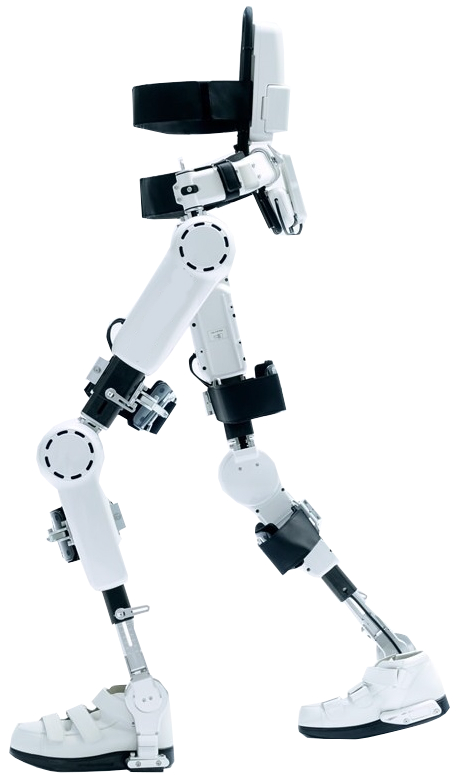
\includegraphics[width=.3\linewidth]{images/fig_01}}%figues de la page de garde


\iflivret
\pagestyle{empty}


%%%%%%%% PAGE DE GARDE COURS
\ifcours
% ==== BANDEAU DES TITRES ==== 
\begin{tikzpicture}[remember picture,overlay]
\node at (current page.north west)
{\begin{tikzpicture}[remember picture,overlay]
\node[anchor=north west,inner sep=0pt] at (0,0) {\includegraphics[width=\paperwidth]{\thechapterimage}};
\draw[anchor=west] (-2cm,-8cm) node [line width=2pt,rounded corners=15pt,draw=ocre,fill=white,fill opacity=0.6,inner sep=40pt]{\strut\makebox[22cm]{}};
\draw[anchor=west] (1cm,-8cm) node {\huge\sffamily\bfseries\color{black} %
\begin{minipage}{1cm}
\rotatebox{90}{\LARGE\sffamily\textsc{\color{ocre}\textbf{\xxnumpartie}}}
\end{minipage} \hfill
\begin{minipage}[c]{14cm}
\begin{titrepartie}
\begin{flushright}
\renewcommand{\baselinestretch}{1.1} 
\Large\sffamily\textsc{\textbf{\xxpartie}}
\renewcommand{\baselinestretch}{1} 
\end{flushright}
\end{titrepartie}
\end{minipage} \hfill
\begin{minipage}[c]{3.5cm}
{\large\sffamily\textsc{\textbf{\color{ocre} \discipline}}}
\end{minipage} 
 };
\end{tikzpicture}};
\end{tikzpicture}
% ==== FIN BANDEAU DES TITRES ==== 


% ==== ONGLET 
\begin{tikzpicture}[overlay]
\node[shape=rectangle, 
      rounded corners = .25 cm,
	  draw= ocre,
	  line width=2pt, 
	  fill = ocre!10,
	  minimum width  = 2.5cm,
	  minimum height = 3cm,] at (18.3cm,0) {};
\node at (17.7cm,0) {\rotatebox{90}{\textbf{\Large\color{ocre}{\classe}}}};
%{};
\end{tikzpicture}
% ==== FIN ONGLET 


\vspace{3.5cm}

\begin{tikzpicture}[remember picture,overlay]
\draw[anchor=west] (-2cm,-6cm) node {\huge\sffamily\bfseries\color{black} %
\begin{minipage}{2cm}
\begin{center}
\LARGE\sffamily\textsc{\color{ocre}\textbf{\xxactivite}}
\end{center}
\end{minipage} \hfill
\begin{minipage}[c]{15cm}
\begin{titrechapitre}
\renewcommand{\baselinestretch}{1.1} 
\Large\sffamily\textsc{\textbf{\xxnumchapitre}}

\Large\sffamily\textsc{\textbf{\xxchapitre}}
\vspace{.5cm}

\renewcommand{\baselinestretch}{1} 
\normalsize\normalfont
\xxcompetences
\end{titrechapitre}
\end{minipage}  };
\end{tikzpicture}
\vfill

\begin{flushright}
\begin{minipage}[c]{.3\linewidth}
\begin{center}
\xxfigures
\end{center}
\end{minipage}\hfill
\begin{minipage}[c]{.6\linewidth}
\startcontents
%\printcontents{}{1}{}
\printcontents{}{1}{}
\end{minipage}
\end{flushright}

\begin{tikzpicture}[remember picture,overlay]
\draw[anchor=west] (4.5cm,-.7cm) node {
\begin{minipage}[c]{.2\linewidth}
\begin{flushright}

\includegraphics[width=2cm]{logoCC}
\end{flushright}
\end{minipage}
\begin{minipage}[c]{.2\linewidth}
\textsl{\xxauteur} \\
\textsl{\classe}
\end{minipage}
 };
\end{tikzpicture}

\newpage
\pagestyle{fancy}

%\newpage
%\pagestyle{fancy}

\else
\fi
%% FIN PAGE DE GARDE DES COURS

%%%%%%%% PAGE DE GARDE TD
\iftd
%\begin{tikzpicture}[remember picture,overlay]
%\node at (current page.north west)
%{\begin{tikzpicture}[remember picture,overlay]
%\draw[anchor=west] (-2cm,-3.25cm) node [line width=2pt,rounded corners=15pt,draw=ocre,fill=white,fill opacity=0.6,inner sep=40pt]{\strut\makebox[22cm]{}};
%\draw[anchor=west] (1cm,-3.25cm) node {\huge\sffamily\bfseries\color{black} %
%\begin{minipage}{1cm}
%\rotatebox{90}{\LARGE\sffamily\textsc{\color{ocre}\textbf{\xxnumpartie}}}
%\end{minipage} \hfill
%\begin{minipage}[c]{13.5cm}
%\begin{titrepartie}
%\begin{flushright}
%\renewcommand{\baselinestretch}{1.1} 
%\Large\sffamily\textsc{\textbf{\xxpartie}}
%\renewcommand{\baselinestretch}{1} 
%\end{flushright}
%\end{titrepartie}
%\end{minipage} \hfill
%\begin{minipage}[c]{3.5cm}
%{\large\sffamily\textsc{\textbf{\color{ocre} \discipline}}}
%\end{minipage} 
% };
%\end{tikzpicture}};
%\end{tikzpicture}

%%%%%%%%%% PAGE DE GARDE TD %%%%%%%%%%%%%%%
%\begin{tikzpicture}[overlay]
%\node[shape=rectangle, 
%      rounded corners = .25 cm,
%	  draw= ocre,
%	  line width=2pt, 
%	  fill = ocre!10,
%	  minimum width  = 2.5cm,
%	  minimum height = 2.5cm,] at (18.5cm,0) {};
%\node at (17.7cm,0) {\rotatebox{90}{\textbf{\Large\color{ocre}{\classe}}}};
%%{};
%\end{tikzpicture}

% PARTIE ET CHAPITRE
%\begin{tikzpicture}[remember picture,overlay]
%\draw[anchor=west] (-1cm,-2.1cm) node {\large\sffamily\bfseries\color{black} %
%\begin{minipage}[c]{15cm}
%\begin{flushleft}
%\xxnumchapitre \\
%\xxchapitre
%\end{flushleft}
%\end{minipage}  };
%\end{tikzpicture}

% BANDEAU EXO
\iflivret % SI LIVRET
\begin{tikzpicture}[remember picture,overlay]
\draw[anchor=west] (-2cm,-3.3cm) node {\huge\sffamily\bfseries\color{black} %
\begin{minipage}{5cm}
\begin{center}
\LARGE\sffamily\color{ocre}\textbf{\textsc{\xxactivite}}

\begin{center}
\xxfigures
\end{center}

\end{center}
\end{minipage} \hfill
\begin{minipage}[c]{12cm}
\begin{titrechapitre}
\renewcommand{\baselinestretch}{1.1} 
\large\sffamily\textbf{\textsc{\xxtitreexo}}

\small\sffamily{\textbf{\textit{\color{black!70}\xxsourceexo}}}
\vspace{.5cm}

\renewcommand{\baselinestretch}{1} 
\normalsize\normalfont
\xxcompetences
\end{titrechapitre}
\end{minipage}};
\end{tikzpicture}
\else % ELSE NOT LIVRET
\begin{tikzpicture}[remember picture,overlay]
\draw[anchor=west] (-2cm,-4.5cm) node {\huge\sffamily\bfseries\color{black} %
\begin{minipage}{5cm}
\begin{center}
\LARGE\sffamily\color{ocre}\textbf{\textsc{\xxactivite}}

\begin{center}
\xxfigures
\end{center}

\end{center}
\end{minipage} \hfill
\begin{minipage}[c]{12cm}
\begin{titrechapitre}
\renewcommand{\baselinestretch}{1.1} 
\large\sffamily\textbf{\textsc{\xxtitreexo}}

\small\sffamily{\textbf{\textit{\color{black!70}\xxsourceexo}}}
\vspace{.5cm}

\renewcommand{\baselinestretch}{1} 
\normalsize\normalfont
\xxcompetences
\end{titrechapitre}
\end{minipage}};
\end{tikzpicture}

\fi

\else   % FIN IF TD
\fi


%%%%%%%% PAGE DE GARDE FICHE
\iffiche
\begin{tikzpicture}[remember picture,overlay]
\node at (current page.north west)
{\begin{tikzpicture}[remember picture,overlay]
\draw[anchor=west] (-2cm,-2.25cm) node [line width=2pt,rounded corners=15pt,draw=ocre,fill=white,fill opacity=0.6,inner sep=40pt]{\strut\makebox[22cm]{}};
\draw[anchor=west] (1cm,-2.25cm) node {\huge\sffamily\bfseries\color{black} %
\begin{minipage}{1cm}
\rotatebox{90}{\LARGE\sffamily\textsc{\color{ocre}\textbf{\xxnumpartie}}}
\end{minipage} \hfill
\begin{minipage}[c]{14cm}
\begin{titrepartie}
\begin{flushright}
\renewcommand{\baselinestretch}{1.1} 
\large\sffamily\textsc{\textbf{\xxpartie} \\} 

\vspace{.2cm}

\normalsize\sffamily\textsc{\textbf{\xxnumchapitre -- \xxchapitre}}
\renewcommand{\baselinestretch}{1} 
\end{flushright}
\end{titrepartie}
\end{minipage} \hfill
\begin{minipage}[c]{3.5cm}
{\large\sffamily\textsc{\textbf{\color{ocre} \discipline}}}
\end{minipage} 
 };
\end{tikzpicture}};
\end{tikzpicture}

\iflivret
\begin{tikzpicture}[overlay]
\node[shape=rectangle, 
      rounded corners = .25 cm,
	  draw= ocre,
	  line width=2pt, 
	  fill = ocre!10,
	  minimum width  = 2.5cm,
	  minimum height = 2.5cm,] at (18.5cm,.5cm) {};
\node at (17.9cm,.5cm) {\rotatebox{90}{\textsf{\textbf{\large\color{ocre}{\classe}}}}};
%{};
\end{tikzpicture}
\else
\begin{tikzpicture}[overlay]
\node[shape=rectangle, 
      rounded corners = .25 cm,
	  draw= ocre,
	  line width=2pt, 
	  fill = ocre!10,
	  minimum width  = 2.5cm,
%	  minimum height = 2.5cm,] at (18.5cm,1.1cm) {};
	  minimum height = 2.5cm,] at (18.6cm,0.5cm) {};
\node at (18cm,0.5cm) {\rotatebox{90}{\textsf{\textbf{\large\color{ocre}{\classe}}}}};
%{};
\end{tikzpicture}

\fi

\else
\fi



\else
\pagestyle{empty}


%%%%%%%% PAGE DE GARDE COURS
\ifcours
% ==== BANDEAU DES TITRES ==== 
\begin{tikzpicture}[remember picture,overlay]
\node at (current page.north west)
{\begin{tikzpicture}[remember picture,overlay]
\node[anchor=north west,inner sep=0pt] at (0,0) {\includegraphics[width=\paperwidth]{\thechapterimage}};
\draw[anchor=west] (-2cm,-8cm) node [line width=2pt,rounded corners=15pt,draw=ocre,fill=white,fill opacity=0.6,inner sep=40pt]{\strut\makebox[22cm]{}};
\draw[anchor=west] (1cm,-8cm) node {\huge\sffamily\bfseries\color{black} %
\begin{minipage}{1cm}
\rotatebox{90}{\LARGE\sffamily\textsc{\color{ocre}\textbf{\xxnumpartie}}}
\end{minipage} \hfill
\begin{minipage}[c]{14cm}
\begin{titrepartie}
\begin{flushright}
\renewcommand{\baselinestretch}{1.1} 
\Large\sffamily\textsc{\textbf{\xxpartie}}
\renewcommand{\baselinestretch}{1} 
\end{flushright}
\end{titrepartie}
\end{minipage} \hfill
\begin{minipage}[c]{3.5cm}
{\large\sffamily\textsc{\textbf{\color{ocre} \discipline}}}
\end{minipage} 
 };
\end{tikzpicture}};
\end{tikzpicture}
% ==== FIN BANDEAU DES TITRES ==== 


% ==== ONGLET 
\begin{tikzpicture}[overlay]
\node[shape=rectangle, 
      rounded corners = .25 cm,
	  draw= ocre,
	  line width=2pt, 
	  fill = ocre!10,
	  minimum width  = 2.5cm,
	  minimum height = 3cm,] at (18.3cm,0) {};
\node at (17.7cm,0) {\rotatebox{90}{\textbf{\Large\color{ocre}{\classe}}}};
%{};
\end{tikzpicture}
% ==== FIN ONGLET 


\vspace{3.5cm}

\begin{tikzpicture}[remember picture,overlay]
\draw[anchor=west] (-2cm,-6cm) node {\huge\sffamily\bfseries\color{black} %
\begin{minipage}{2cm}
\begin{center}
\LARGE\sffamily\textsc{\color{ocre}\textbf{\xxactivite}}
\end{center}
\end{minipage} \hfill
\begin{minipage}[c]{15cm}
\begin{titrechapitre}
\renewcommand{\baselinestretch}{1.1} 
\Large\sffamily\textsc{\textbf{\xxnumchapitre}}

\Large\sffamily\textsc{\textbf{\xxchapitre}}
\vspace{.5cm}

\renewcommand{\baselinestretch}{1} 
\normalsize\normalfont
\xxcompetences
\end{titrechapitre}
\end{minipage}  };
\end{tikzpicture}
\vfill

\begin{flushright}
\begin{minipage}[c]{.3\linewidth}
\begin{center}
\xxfigures
\end{center}
\end{minipage}\hfill
\begin{minipage}[c]{.6\linewidth}
\startcontents
%\printcontents{}{1}{}
\printcontents{}{1}{}
\end{minipage}
\end{flushright}

\begin{tikzpicture}[remember picture,overlay]
\draw[anchor=west] (4.5cm,-.7cm) node {
\begin{minipage}[c]{.2\linewidth}
\begin{flushright}

\includegraphics[width=2cm]{logoCC}
\end{flushright}
\end{minipage}
\begin{minipage}[c]{.2\linewidth}
\textsl{\xxauteur} \\
\textsl{\classe}
\end{minipage}
 };
\end{tikzpicture}

\newpage
\pagestyle{fancy}

%\newpage
%\pagestyle{fancy}

\else
\fi
%% FIN PAGE DE GARDE DES COURS

%%%%%%%% PAGE DE GARDE TD
\iftd
%\begin{tikzpicture}[remember picture,overlay]
%\node at (current page.north west)
%{\begin{tikzpicture}[remember picture,overlay]
%\draw[anchor=west] (-2cm,-3.25cm) node [line width=2pt,rounded corners=15pt,draw=ocre,fill=white,fill opacity=0.6,inner sep=40pt]{\strut\makebox[22cm]{}};
%\draw[anchor=west] (1cm,-3.25cm) node {\huge\sffamily\bfseries\color{black} %
%\begin{minipage}{1cm}
%\rotatebox{90}{\LARGE\sffamily\textsc{\color{ocre}\textbf{\xxnumpartie}}}
%\end{minipage} \hfill
%\begin{minipage}[c]{13.5cm}
%\begin{titrepartie}
%\begin{flushright}
%\renewcommand{\baselinestretch}{1.1} 
%\Large\sffamily\textsc{\textbf{\xxpartie}}
%\renewcommand{\baselinestretch}{1} 
%\end{flushright}
%\end{titrepartie}
%\end{minipage} \hfill
%\begin{minipage}[c]{3.5cm}
%{\large\sffamily\textsc{\textbf{\color{ocre} \discipline}}}
%\end{minipage} 
% };
%\end{tikzpicture}};
%\end{tikzpicture}

%%%%%%%%%% PAGE DE GARDE TD %%%%%%%%%%%%%%%
%\begin{tikzpicture}[overlay]
%\node[shape=rectangle, 
%      rounded corners = .25 cm,
%	  draw= ocre,
%	  line width=2pt, 
%	  fill = ocre!10,
%	  minimum width  = 2.5cm,
%	  minimum height = 2.5cm,] at (18.5cm,0) {};
%\node at (17.7cm,0) {\rotatebox{90}{\textbf{\Large\color{ocre}{\classe}}}};
%%{};
%\end{tikzpicture}

% PARTIE ET CHAPITRE
%\begin{tikzpicture}[remember picture,overlay]
%\draw[anchor=west] (-1cm,-2.1cm) node {\large\sffamily\bfseries\color{black} %
%\begin{minipage}[c]{15cm}
%\begin{flushleft}
%\xxnumchapitre \\
%\xxchapitre
%\end{flushleft}
%\end{minipage}  };
%\end{tikzpicture}

% BANDEAU EXO
\iflivret % SI LIVRET
\begin{tikzpicture}[remember picture,overlay]
\draw[anchor=west] (-2cm,-3.3cm) node {\huge\sffamily\bfseries\color{black} %
\begin{minipage}{5cm}
\begin{center}
\LARGE\sffamily\color{ocre}\textbf{\textsc{\xxactivite}}

\begin{center}
\xxfigures
\end{center}

\end{center}
\end{minipage} \hfill
\begin{minipage}[c]{12cm}
\begin{titrechapitre}
\renewcommand{\baselinestretch}{1.1} 
\large\sffamily\textbf{\textsc{\xxtitreexo}}

\small\sffamily{\textbf{\textit{\color{black!70}\xxsourceexo}}}
\vspace{.5cm}

\renewcommand{\baselinestretch}{1} 
\normalsize\normalfont
\xxcompetences
\end{titrechapitre}
\end{minipage}};
\end{tikzpicture}
\else % ELSE NOT LIVRET
\begin{tikzpicture}[remember picture,overlay]
\draw[anchor=west] (-2cm,-4.5cm) node {\huge\sffamily\bfseries\color{black} %
\begin{minipage}{5cm}
\begin{center}
\LARGE\sffamily\color{ocre}\textbf{\textsc{\xxactivite}}

\begin{center}
\xxfigures
\end{center}

\end{center}
\end{minipage} \hfill
\begin{minipage}[c]{12cm}
\begin{titrechapitre}
\renewcommand{\baselinestretch}{1.1} 
\large\sffamily\textbf{\textsc{\xxtitreexo}}

\small\sffamily{\textbf{\textit{\color{black!70}\xxsourceexo}}}
\vspace{.5cm}

\renewcommand{\baselinestretch}{1} 
\normalsize\normalfont
\xxcompetences
\end{titrechapitre}
\end{minipage}};
\end{tikzpicture}

\fi

\else   % FIN IF TD
\fi


%%%%%%%% PAGE DE GARDE FICHE
\iffiche
\begin{tikzpicture}[remember picture,overlay]
\node at (current page.north west)
{\begin{tikzpicture}[remember picture,overlay]
\draw[anchor=west] (-2cm,-2.25cm) node [line width=2pt,rounded corners=15pt,draw=ocre,fill=white,fill opacity=0.6,inner sep=40pt]{\strut\makebox[22cm]{}};
\draw[anchor=west] (1cm,-2.25cm) node {\huge\sffamily\bfseries\color{black} %
\begin{minipage}{1cm}
\rotatebox{90}{\LARGE\sffamily\textsc{\color{ocre}\textbf{\xxnumpartie}}}
\end{minipage} \hfill
\begin{minipage}[c]{14cm}
\begin{titrepartie}
\begin{flushright}
\renewcommand{\baselinestretch}{1.1} 
\large\sffamily\textsc{\textbf{\xxpartie} \\} 

\vspace{.2cm}

\normalsize\sffamily\textsc{\textbf{\xxnumchapitre -- \xxchapitre}}
\renewcommand{\baselinestretch}{1} 
\end{flushright}
\end{titrepartie}
\end{minipage} \hfill
\begin{minipage}[c]{3.5cm}
{\large\sffamily\textsc{\textbf{\color{ocre} \discipline}}}
\end{minipage} 
 };
\end{tikzpicture}};
\end{tikzpicture}

\iflivret
\begin{tikzpicture}[overlay]
\node[shape=rectangle, 
      rounded corners = .25 cm,
	  draw= ocre,
	  line width=2pt, 
	  fill = ocre!10,
	  minimum width  = 2.5cm,
	  minimum height = 2.5cm,] at (18.5cm,.5cm) {};
\node at (17.9cm,.5cm) {\rotatebox{90}{\textsf{\textbf{\large\color{ocre}{\classe}}}}};
%{};
\end{tikzpicture}
\else
\begin{tikzpicture}[overlay]
\node[shape=rectangle, 
      rounded corners = .25 cm,
	  draw= ocre,
	  line width=2pt, 
	  fill = ocre!10,
	  minimum width  = 2.5cm,
%	  minimum height = 2.5cm,] at (18.5cm,1.1cm) {};
	  minimum height = 2.5cm,] at (18.6cm,0.5cm) {};
\node at (18cm,0.5cm) {\rotatebox{90}{\textsf{\textbf{\large\color{ocre}{\classe}}}}};
%{};
\end{tikzpicture}

\fi

\else
\fi



\fi
\setlength{\columnseprule}{.1pt}

\pagestyle{fancy}
\thispagestyle{plain}

\ifprof
\vspace{5.1cm}
\else
\vspace{5.2cm}
\fi

\def\columnseprulecolor{\color{ocre}}
\setlength{\columnseprule}{0.4pt} 

%%%%%%%%%%%%%%%%%%%%%%%

\setcounter{exo}{0}



\ifprof
\else
\begin{multicols}{2}
\fi

\section*{Mise en situation -- Assurer le mouvement vertical}
\ifprof
\else

\ifprof
\else
\noindent
\begin{tabular}{m{.6\linewidth}m{.3\linewidth}}
L’exosquelette est un appareil qui apporte à un être humain des capacités qu’il ne possède pas ou qu’il a perdues à cause d’un accident. Ce type d’appareil peut permettre à une personne de soulever des charges lourdes et diminuer considérablement les efforts à fournir sans la moindre fatigue. Après avoir revêtu un exosquelette adapté à sa morphologie et à sa taille, l’utilisateur peut faire ses mouvements en bénéficiant
d’une grande fluidité.
& 
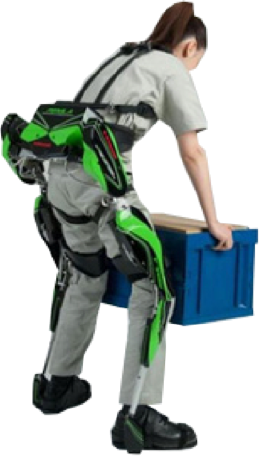
\includegraphics[width=\linewidth]{images/fig_02}

\end{tabular}



\begin{center}
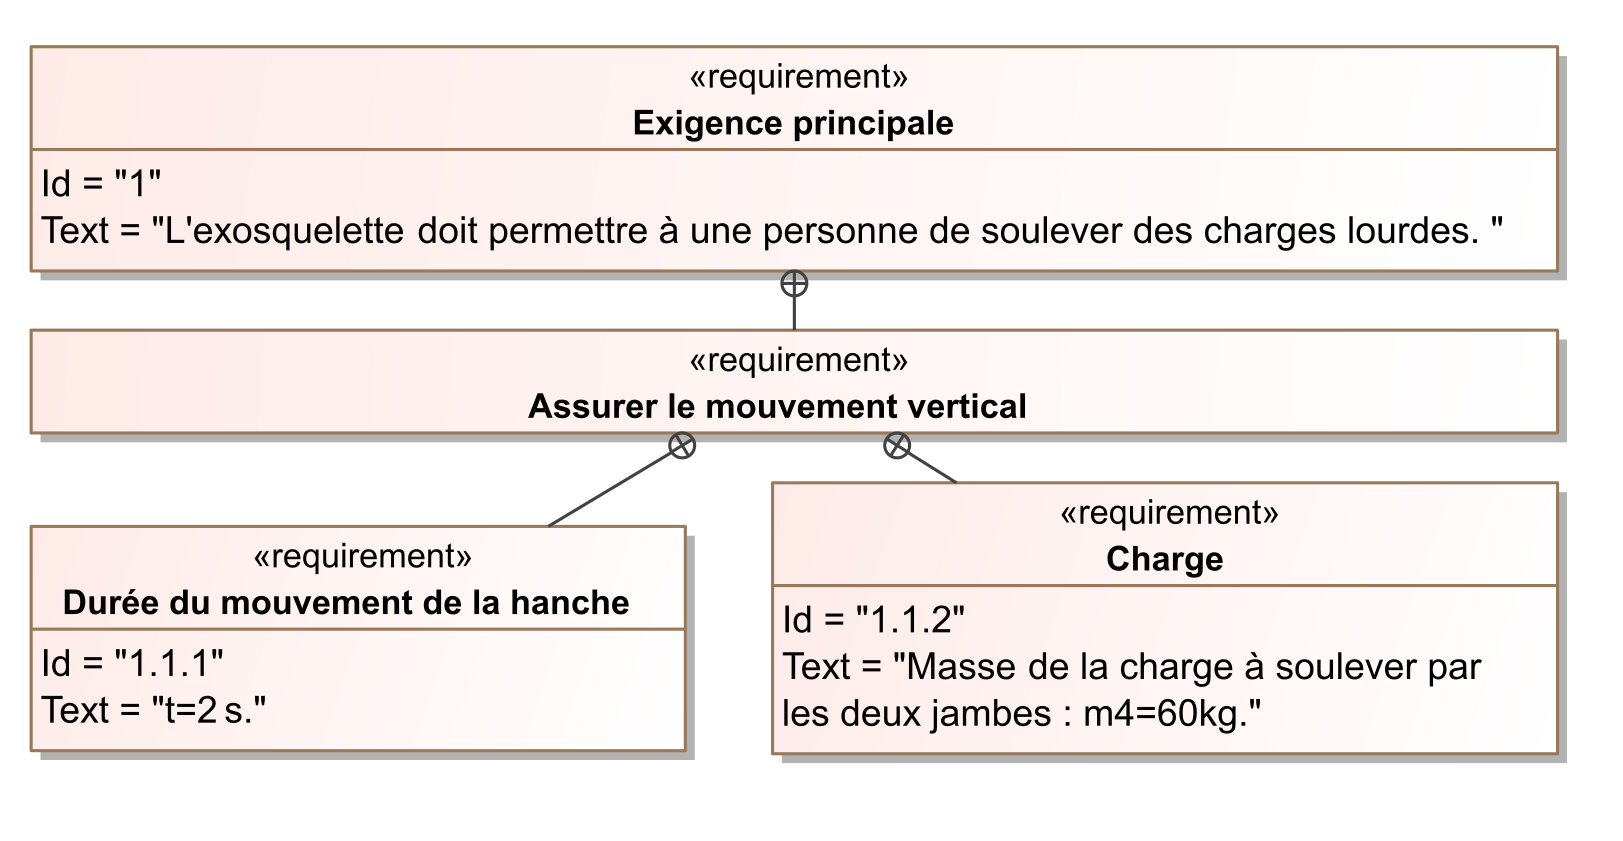
\includegraphics[width=\linewidth]{images/Exigences}
%\textit{}
\end{center}
\fi

%\subsection*{}
\fi
\begin{obj}
Proposer un modèle de connaissance des éléments réalisant l’exigence fonctionnelle <<~assurer le mouvement vertical~>> puis valider les performances attendues listées par le cahier des charges.
\end{obj}



%\subsection*{Élaboration du modèle géométrique direct et du modèle articulaire inverse}
%\begin{obj}
%Élaborer la commande du moteur pilotant le genou à partir d’un mouvement défini dans l’espace
%opérationnel puis converti dans l’espace articulaire.
%\end{obj}
%
%\ifprof
%\else
%L’étude se limite au passage de la position accroupie à la position relevée de l’exosquelette. Lors de ce passage,
%le point $O_2$ est en mouvement de translation verticale suivant la direction $\axe{O_0}{{z_0}}$ et sa vitesse de déplacement
%évolue selon une loi trapézoïdale. Un modèle plan de la chaîne cinématique ouverte représente la partie inférieure
%de l’exosquelette en position debout et fléchie.
%
%
%\begin{center}
%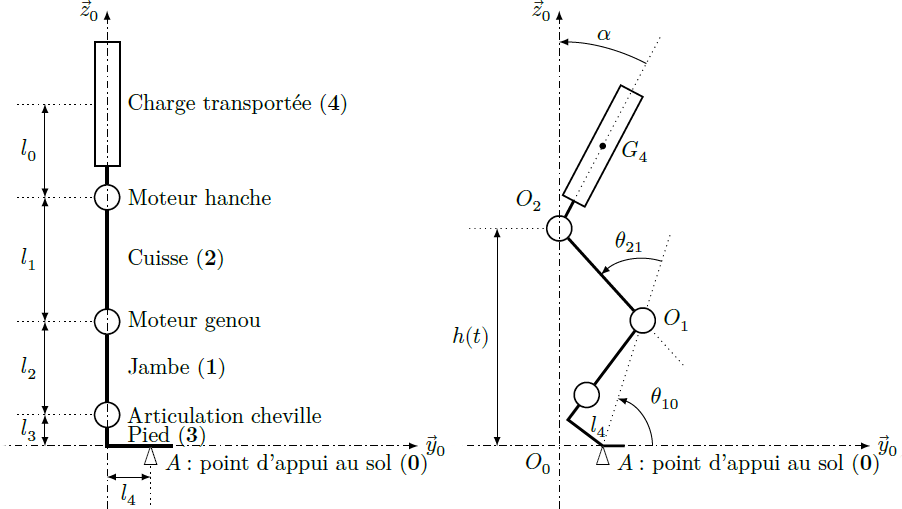
\includegraphics[width=\linewidth]{images/fig_03}
%%\textit{}
%\end{center}
%
%
%%Selon le cahier des charges, pour assurer une bonne synchronisation des axes, l’exigence de précision statique suite à une entrée de type échelon, de type rampe ou de type accélération doit être inférieure à 1\%.
%
%
%On donne le paramétrage du modèle proposé. 
%
%\begin{center}
%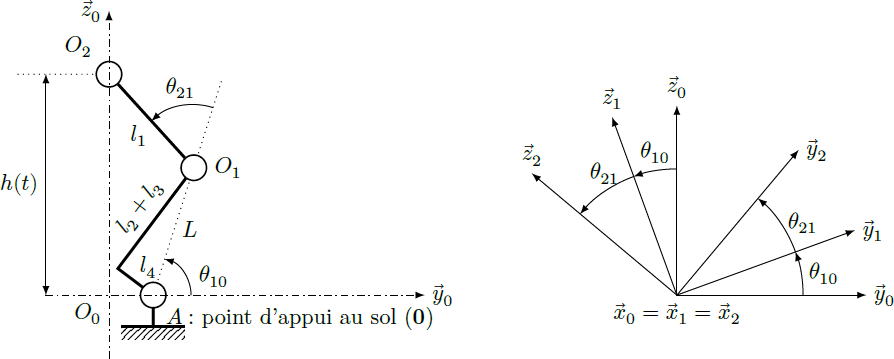
\includegraphics[width=\linewidth]{images/fig_04}
%%\textit{}
%\end{center}
%
%\textbf{Hypothèses : }
%\begin{itemize}
%\item le référentiel lié au repère $\mathcal{R}_0\repere{A}{x_0}{y_0}{z_0}$ est galiléen et est fixe par rapport à la terre;
%\item le point $O_2$ représentant la hanche se déplace verticalement selon la direction $\axe{O_0}{z_0}$;
%\item l’angle $\alpha$ entre la charge transportée et la verticale $\vect{z_0}$ reste constant;
%\item le point d’appui $A$ du pied sur le sol est considéré fixe par rapport à la terre;
%\item lors du mouvement étudié la jambe (1) reste perpendiculaire au pied (3).
%\end{itemize}
%
%\textbf{Données : }
%\begin{itemize}
%\item $\theta_{10}=\angl{y_0}{y_1}=\angl{z_0}{z_1}$;
%\item $\theta_{21}=\angl{y_1}{y_2}=\angl{z_1}{z_2}$;
%\item $\alpha=\text{constante}$;
%\item $L=\sqrt{\left(l_2+l_3\right)^2+l_4^2}$.
%\end{itemize}
%
%\fi
%
%\subparagraph{}\textit{Déterminer littéralement les coordonnées opérationnelles $l_4$ et $h(t)$ en fonction des coordonnées articulaires $\theta_{10}$, $\theta_{21}$ et des paramètres dimensionnels $L$ et $l_1$.}
%\ifprof
%\begin{corrige}
%On a $\vect{A O_1}+\vect{O_1 O_2}+\vect{O_2 O_0}+\vect{O_0 A}=\vect{0}$ soit 
%$L\vect{y_1}+l_1\vect{y_2}-h(t)\vect{z_0}+l_4\vect{y_0}=\vect{0}$. 
%En projetant sur $\vect{y_0}$ et $\vect{z_0}$ on a :
%$$
%\left\{
%\begin{array}{l}
%L\cos\theta_{10} +l_1\cos\left(\theta_{10}+\theta_{21}\right)+l_4={0} \\
%L\sin\theta_{10}  +l_1\sin\left(\theta_{10}+\theta_{21}\right)-h(t) ={0} \\
%\end{array}
%\right.
%$$
%
%En projetant sur $\vect{y_1}$ et $\vect{z_1}$ on a :
%$$
%\left\{
%\begin{array}{l}
%L+l_1\cos\theta_{21}-h(t)\sin\theta_{10}+l_4\cos\theta_{10}={0} \\
%l_1\sin\theta_{21}-h(t)\cos\theta_{10}-l_4\sin\theta_{10}={0}
%\end{array}
%\right.
%$$
%
%
%\end{corrige}
%\else
%\fi
%
%
%\subparagraph{}\textit{Déterminer le modèle articulaire inverse $\theta_{10}$ et $\theta_{21}$ en fonction de $l_1$, $l_4$, $L$ et $h(t)$.}
%\ifprof
%\begin{corrige}
%Pour exprimer $\theta_{10}$, on peut utiliser le premier système d'équation : 
%$$
%\left\{
%\begin{array}{l}
%L\cos\theta_{10}+l_4 =-l_1\cos\left(\theta_{10}+\theta_{21}\right) \\
%L\sin\theta_{10}-h(t)  =-l_1\sin\left(\theta_{10}+\theta_{21}\right) \\
%\end{array}
%\right.
%$$
%En élevant les expressions au carré, on a alors : 
%$
%l_1^2 = \left(L\cos\theta_{10}+l_4 \right)^2+ \left(L\sin\theta_{10}-h(t)\right)^2
%$
%$
%\Leftrightarrow 
%l_1^2 = L^2+l_4^2 +h(t)^2+2Ll_4\cos\theta_{10} -2Lh(t)\sin\theta_{10}
%$
%
%$
%\Leftrightarrow 
%\dfrac{l_1^2 - L^2-l_4^2 -h(t)^2}{2L}=l_4\cos\theta_{10} -h(t)\sin\theta_{10}
%$
%
%En utilisant l'indication, on a : 
%$$
%\dfrac{l_4}{\sqrt{l_4^2 + h(t)^2}}\cos\theta_{10} +\dfrac{-h(t)}{\sqrt{l_4^2 + h(t)^2}}\sin\theta_{10}=\dfrac{l_1^2 - L^2-l_4^2 -h(t)^2}{2L{\sqrt{l_4^2 + h(t)^2}}}
%$$
%En conséquence, on pose $\cos\varphi=\dfrac{l_4}{\sqrt{l_4^2 + h(t)^2}}$ et 
%$\sin\varphi = \dfrac{-h(t)}{\sqrt{l_4^2 + h(t)^2}}$. 
%En conséquences %$\tan\varphi = \dfrac{\dfrac{-h(t)}{\sqrt{l_4^2 + h(t)^2}}}{\dfrac{l_4}{\sqrt{l_4^2 + h(t)^2}}}=\dfrac{-h(t)}{l_4}$.
%$\tan\varphi =\dfrac{-h(t)}{l_4}$.
%
%
%Par suite, $\cos\left( \theta_{10} - \varphi \right) =\dfrac{l_1^2 - L^2-l_4^2 -h(t)^2}{2L{\sqrt{l_4^2 + h(t)^2}}}$. On a donc 
%$\theta_{10} =\arccos \left( \dfrac{l_1^2 - L^2-l_4^2 -h(t)^2}{2L{\sqrt{l_4^2 + h(t)^2}}}\right) + \varphi$.
%
%
%Au final, 
%$$\theta_{10} =\arccos \left( \dfrac{l_1^2 - L^2-l_4^2 -h(t)^2}{2L{\sqrt{l_4^2 + h(t)^2}}}\right) + \arctan\left(\dfrac{-h(t)}{l_4} \right).$$
%
%Pour exprimer  $\theta_{21}$ on réutilise le premier système d'équations :
%$
%\left\{
%\begin{array}{l}
%-l_4 =l_1\cos\left(\theta_{10}+\theta_{21}\right) + L\cos\theta_{10} \\
%h(t)  =l_1\sin\left(\theta_{10}+\theta_{21}\right) + L\sin\theta_{10}\\
%\end{array}
%\right.
%$
%
%On a alors 
%$l_4 ^2 +h(t)^2= L^2 + l_1^2 + 2l_1L\left(\cos\theta_{10}\cos\left(\theta_{10}+\theta_{21}\right) +\sin\left(\theta_{10}+\theta_{21}\right) \sin\theta_{10}\right)$.
%En conséquences, 
%$\dfrac{l_4 ^2 +h(t)^2- L^2 - l_1^2}{2l_1L} = \cos\theta_{10}\cos\left(\theta_{10}+\theta_{21}\right) +\sin\left(\theta_{10}+\theta_{21}\right) \sin\theta_{10}$
%$= \cos\left(\theta_{10}+\theta_{21}-\theta_{10}\right) $.
%D'où $\theta_{21}=\arccos\left(\dfrac{l_4 ^2 +h(t)^2- L^2 - l_1^2}{2l_1L}  \right)$.
%\end{corrige}
%
%
%\else
%\fi
%
%\ifprof
%\else
%\begin{methode}
%Lorsqu'on a une équation de la forme $A\cos\theta_{10}+B\sin\theta_{10}=C$. On peut normer cette équation en la mettant sous la forme $\dfrac{A}{\sqrt{A^2+B^2}}\cos\theta_{10}+\dfrac{B}{\sqrt{A^2+B^2}}\sin\theta_{10}=\dfrac{C}{\sqrt{A^2+B^2}}$.
%On pose alors $\cos\varphi = \dfrac{A}{\sqrt{A^2+B^2}}$ et $\sin\varphi=\dfrac{B}{\sqrt{A^2+B^2}}$. On a alors $\cos\left( \theta_{10} - \varphi \right)=\dfrac{C}{\sqrt{A^2+B^2}}$.
%\end{methode}
%\fi
%
%\subsection*{Élaboration du modèle cinématique}
%\begin{obj}
%En vue de dimensionner le moteur du genou, déterminer la vitesse articulaire en fonction de la  vitesse opérationnelle.
%\end{obj}
%
%\subparagraph{}\textit{Déterminer à partir du modèle articulaire inverse la vitesse angulaire 
%$\theta_{21}$ en fonction de $h(t)$, $\dot{h}(t)$, $l_1$, $L$ et $\sin\theta_{21}$.}
%\ifprof
%\begin{corrige}
%On a vu que $\cos\theta_{21}=\dfrac{l_4 ^2 +h(t)^2- L^2 - l_1^2}{2l_1L}  $.
%En dérivant, on a donc $- \dot{\theta}_{21} \sin\theta_{21}=\dfrac{2\dot{h}(t)h(t)}{2l_1L}$.
%Au final,  $\dot{\theta}_{21} =-\dfrac{\dot{h}(t)h(t)}{l_1L\sin\theta_{21}}$.
%\end{corrige}
%\else
%\fi
%
%\ifprof
%\else
%Un modèle multiphysique a permis de déterminer les conditions suivantes correspondant à la vitesse maximale : $t=\SI{1,5}{s}$, $h(t=1,5)=\SI{0,829}{m}$, $\dot{h}(t=1,5)=\SI{0,422}{m.s^{-1}}$ et $\theta_{21} = 55,9\degres$. Les longueurs $l_1$ et $L$ valent
%respectivement \SI{43,1}{cm} et \SI{51,8}{cm}. Le réducteur de vitesse utilisé a un rapport de réduction égal à $r=\dfrac{1}{120}$.
%\fi
%
%\subparagraph{}\textit{Déterminer la valeur maximale de la vitesse angulaire $\dot{\theta}_{21}$ et $\text{rad s}^{-1}$ puis celle de la fréquence de rotation d’un moteur de genou en $\text{tr min}^{-1}$.}
%\ifprof
%\begin{corrige}
%On a : $\dot{\theta}_{21} =-\dfrac{0,422 \times 0,829}{0,431\times 0,518\sin \left(55,9\right)}\simeq -\SI{1,89}{rad.s^{-1}}$. Soit une fréquence de rotation du moteur de \SI{2168}{tr.min^{-1}}.
%\end{corrige}
%\else
%\fi


\subsection*{Élaboration du modèle dynamique}

\begin{obj}
Dimensionner le moteur situé au niveau d’un genou permettant à l’exosquelette de soulever une masse de \SI{60}{kg} de la position accroupie à la position debout.
\end{obj}
\ifprof
\else
Ces calculs visent à déterminer l’équation dynamique qui permet d’obtenir le couple moteur (minimal) en fonction des caractéristiques géométriques et massique de la charge à soulever ainsi que des conditions d’utilisation.
Le modèle d’étude est celui représenté à la figure suivante correspondant au modèle d’étude plan position fléchie.
\begin{center}
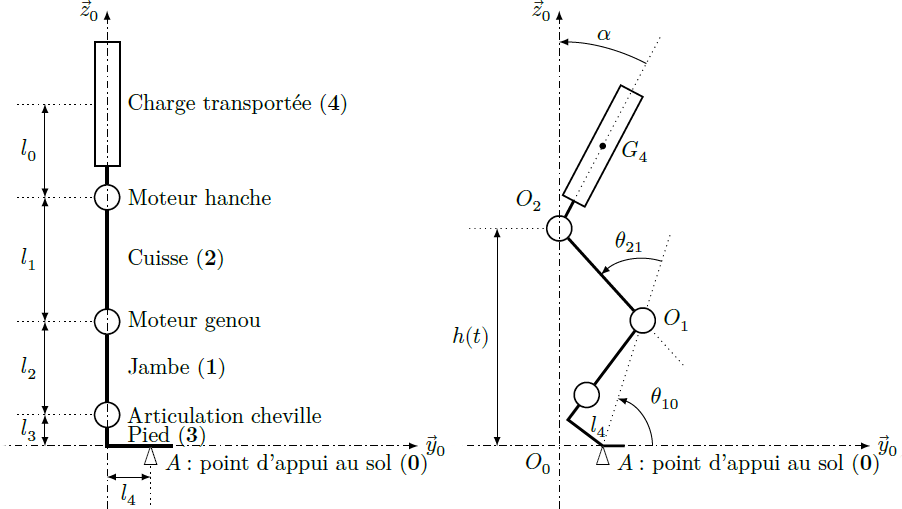
\includegraphics[width=\linewidth]{images/fig_03}
%\textit{}
\end{center}

\begin{center}
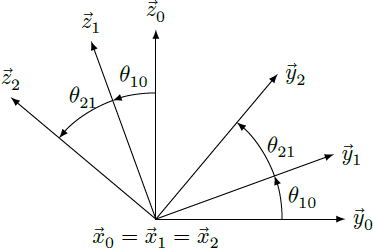
\includegraphics[width=.5\linewidth]{images/fig_14}
%\textit{}
\end{center}


\noindent\textbf{Hypothèses :}
\begin{itemize}
\item L’étude est modélisable dans le plan.
\item Toutes les liaisons sont supposées parfaites.
\item Les inerties des pièces sont négligées sauf la masse de la charge à soulever.
\item L’angle $\alpha$ entre la charge transportée et la verticale$\vect{z_0}$ reste constant.
\item $G_4$, centre de gravité de la charge transportée (4), reste en permanence à la verticale du point $A$ d’appui au sol.
\end{itemize}

\noindent\textbf{Données :}
\begin{itemize}
\item $\vect{O_1G_4}=\lambda(t)\vect{z_0}-L\cos\theta_{10}\vect{y_0}$;
\item Accélération de la pesanteur $g=\SI{9,81}{m.s^{-2}}$;
\item Longueur de la cuisse $l_1 = \SI{43,1}{cm}$.
\item Longueur de la jambe $l_2 = \SI{43,3}{cm}$.
\item Longueur de l'articulation de la cheville à la plante arrière du pied $l_3 = \SI{6,9}{cm}$.
\item Longueur de la plante arrière du pied au point d’appui sur le sol $l_4 = \SI{13}{cm}$.
\item Longueur $\vect{O_0O_1}=L\vect{y_1}$ avec $L=\SI{51,8}{cm}$.
\item Rapport de réduction : $r=\dfrac{1}{120}$.
\end{itemize}

On note E=\{cuisse(2)+charge transportée(4)\}. 

\fi

\subparagraph{} \textit{Donner qualitativement le mouvement de 4 par rapport à 0. Tracer le graphe de structure du système.}

\ifprof
\begin{corrige}
Étant donné que l'on souhaite que l'angle $\alpha$ reste constant pendant la levée d'une charge, le mouvement de 4 sera donc un mouvement de translation rectiligne.  

\begin{center}
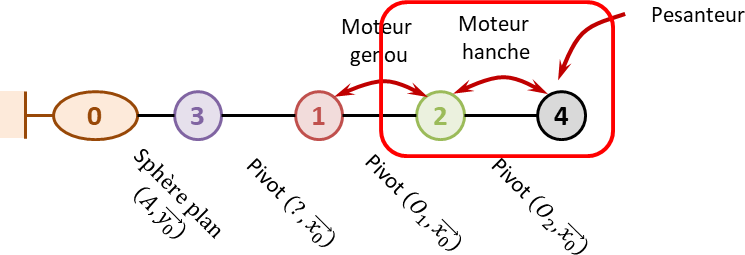
\includegraphics[width=.7\linewidth]{images/cor_00}
\end{center}
\end{corrige}
\else
\fi


\subparagraph{} \textit{Déterminer $\vectmc{O_1}{E}{0}\cdot \vect{x_0}$ en fonction de $m_4$, $\dot{h}(t)$, $L$ et $\cos\theta_{10}$.}

\ifprof
\begin{corrige}
$E$ étant en translation, on a $\vectmc{G_4}{E}{0}=\vect{0}$. On a alors 
 $\vectmc{O_1}{E}{0}=\vectmc{G_4}{E}{0}+\vect{O_1G_4}\wedge\vectrc{E}{0}$.

Par ailleurs, $\vectrc{E}{0}=m_4\vectv{G_4}{E}{0} = m_4\dot{h}(t)\vect{z_0}$. 

On a donc :
$ \vectmc{O_1}{E}{0}\cdot \vect{x_0} 
= \left(\left( \lambda(t)\vect{z_0}-L\cos\theta_{10}\vect{y_0}\right)\wedge m_4\dot{h}(t)\vect{z_0}\right) \cdot \vect{x_0}
=  -Lm_4\cos\theta_{10}\dot{h}(t)$.
 
 
\end{corrige}
\else
\fi




\subparagraph{} \textit{Déduire $\vectmd{O_1}{E}{0}\cdot \vect{x_0}$ en fonction de $m_4$, $\ddot{h}(t)$, $L$ et $\cos\theta_{10}$.}

\ifprof
\begin{corrige}
\subsubsection*{Méthode 1 -- Calcul de $\vectmd{G_4}{E}{0}$ et déplacement}
On a $\vectmd{G_4}{E}{0}= \dfrac{\dd \vectmc{G_4}{E}{0}}{\dd t}= \vect{0}$. En conséquences, 
$ \vectmd{O_1}{E}{0}\cdot \vect{x_0} 
= \left(\left( \lambda(t)\vect{z_0}-L\cos\theta_{10}\vect{y_0}\right)\wedge m_4\ddot{h}(t)\vect{z_0}\right) \cdot \vect{x_0} =  -Lm_4\cos\theta_{10}\ddot{h}(t)$.

\subsubsection*{Méthode 2 -- Calcul de $\vectmd{O_1}{E}{0}$}
On a aussi $\vectmd{O_1}{E}{0} = \left(\dfrac{d \vectmc{O_1}{E}{0}}{\dd t}\right)+m_4\vect{V\left(O_1/0\right)}\wedge\vectv{G_4}{E}{0} $. 

Par suite on a 
$\left(\vectv{O_1}{E}{0}\wedge\vectv{G_4}{E}{0}\right)\vect{x_0}=
\left(\left( L\vect{y_1}\wedge \dot{\theta}_{10} \vect{x_0} \right) \wedge\dot{h}(t)\vect{z_0}\right)\vect{x_0} $

$= \left( -L\dot{\theta}_{10} \vect{z_1} \wedge\dot{h}(t)\vect{z_0}\right)\vect{x_0} $ 

$= -L\dot{\theta}_{10} \dot{h}(t) \sin \theta_{10} $. 

Enfin, 
 $\vectmd{O_1}{E}{0}\cdot\vect{x_0}=-Lm_4\cos\theta_{10}\ddot{h}(t)+Lm_4\dot{\theta}_{10}\sin\theta_{10}\dot{h}(t)-m_4L\dot{\theta}_{10} \dot{h}(t) \sin \theta_{10}$
 $=-Lm_4\cos\theta_{10}\ddot{h}(t)$.
 
\end{corrige}

\else
\fi

\ifprof
\else
La loi d'évolution de la vitesse de la hanche est donnée à la figure suivante. 

\begin{center}
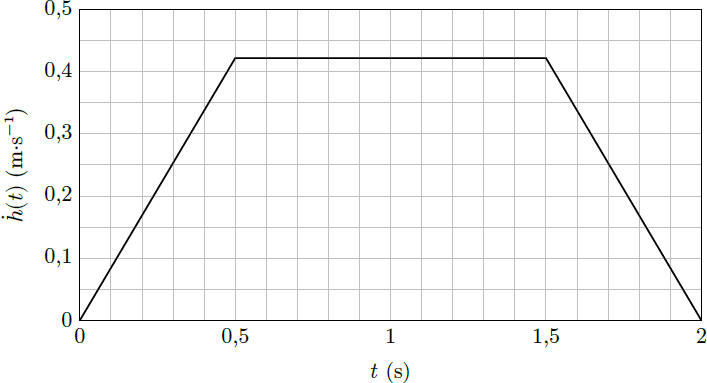
\includegraphics[width=.8\linewidth]{images/fig_11}
%\textit{}
\end{center}
\fi

\subparagraph{} \textit{Déterminer l’expression littérale du couple $C_r$ exercé par l’arbre de sortie du réducteur sur le genou imposé par la loi d’évolution de la hanche et calculer numériquement ce couple pour une valeur de $\theta_{10}$ égale à
54,5\degres correspondant à la valeur maximale du couple.}

\ifprof
\begin{corrige}
\begin{itemize}
\item On isole l'ensemble $E$.
\item On réalise le bilan des actions mécaniques : 
\begin{itemize}
\item action de la liaison pivot : $\torseurstat{T}{1}{E}=\torseurl{\vectf{1}{E}}{\vectm{O_1}{1}{E}}{O_1}$ avec $\vectm{O_1}{1}{E}\cdot \vect{x_0}=0$;
\item action du réducteur: $\torseurstat{T}{1_r}{E}=\torseurl{\vect{0}}{C_r \vect{x_0}}{O_1}$ avec $\vectm{O_1}{1}{E}\cdot \vect{x_0}=0$;
\item action de la pesanteur : 
$\torseurstat{T}{\text{pes}}{E}=\torseurl{-m_4g\vect{z_0}}{\vect{0}}{G_4}$. On a alors 
$\vectm{O_1}{\text{pes}}{E}\cdot \vect{x_0}$ $=\vectm{G_4}{\text{pes}}{E}\cdot \vect{x_0}+\left(\vect{O_1G_4}\wedge -m_4g\vect{z_0} \right)\cdot \vect{x_0}$  
$=\left(\left(\lambda(t)\vect{z_0}-L\cos\theta_{10}\vect{y_0}\right)\wedge -m_4g\vect{z_0} \right)\cdot \vect{x_0}$ 
$=\left(-L\cos\theta_{10}\vect{y_0}\wedge -m_4g\vect{z_0}\right)\cdot \vect{x_0}$ $= m_4gL\cos\theta_{10}$.
\end{itemize}
\item $E$ étant en pivot d'axe $\axe{O_1}{{x_1}}$, on applique le théorème du moment dynamique en $O_1$ en projection sur $\vect{x_1}$ :
$-Lm_4\cos\theta_{10}\ddot{h}(t) =C_r +m_4gL\cos\theta_{10}$
$ \Leftrightarrow C_r=-m_4 L \cos\theta_{10} \left(g+\ddot{h}(t)\right) $. 
\end{itemize}

En réalisant l'application numérique, on a : $C_r = - 60 \times 51,8\times 10^{-2}\times \cos 54,5 \left(9,81 +\dfrac{0,425}{0,5} \right) \simeq \SI{190,5}{Nm} $.


\end{corrige}

\else
\fi

\subparagraph{} \textit{Calculer le couple $C_m$ au niveau de l’arbre moteur du genou en prenant un facteur de perte $\eta = 0,75$ (estimé à l’aide du modèle multiphysique).}
\ifprof
\begin{corrige}
En régime permanent, on a $\eta=\dfrac{C_r \omega_r}{C_m \omega_m}=r\dfrac{C_r}{C_m}$ et $C_m = \dfrac{r}{\eta}C_r=\dfrac{1}{0,75\times 120} \times 190,5 \simeq \SI{2,12}{Nm}$.
\end{corrige}
\else
\fi




\subparagraph{} \textit{Expliquer en moins de 5 lignes comment estimer un rendement à partir d'un modèle multiphysique.}
\ifprof
\begin{corrige}
Si on en avait la possibilité, il faudrait mettre un capteur de puissance au niveau de la commande (mesure de la vitesse et du couple de commande) puis un capteur de puissance au niveau de la charge (mesure de vitesse et du couple en sortie au niveau du genou). Le rendement peut s'observer en régime permanent en faisant le rapport des puissances. 
Pour observer une perte de rendement, il est nécessaire que soient modélisées les actions de frottement.
\end{corrige}
\else
\fi

\subsection*{Validation du dimensionnement du moteur}
\begin{obj}
Vérifier que le moteur choisi convient pour une utilisation intensive comprenant 4 cycles par minute
de descente suivie d’une montée.
\end{obj}

\ifprof
\else

Le cycle suivant obtenu à l’aide du modèle multiphysique de représente l’évolution du couple moteur,
et ce en tenant compte du moment d’inertie du rotor, sur un cycle de période $T=\SI{15}{s}$.


\noindent Quatre phases sont définies sur cette période :
\begin{itemize}
\item phase 1 pour $0 \leq t < \SI{2}{s}$, valeur efficace du couple moteur $C_1 = \SI{0,838}{Nm}$ ;
\item phase 2 pour $2 \leq t < \SI{4}{s}$, couple moteur constant $C_2 = -\SI{0,912}{Nm}$ ;
\item phase 3 pour $4 \leq t < \SI{6}{s}$, valeur efficace du couple moteur $C_3 = \SI{0,838}{Nm}$;
\item phase 4 pour $6 \leq t < \SI{15}{s}$, couple moteur nul.
\end{itemize}



\begin{center}
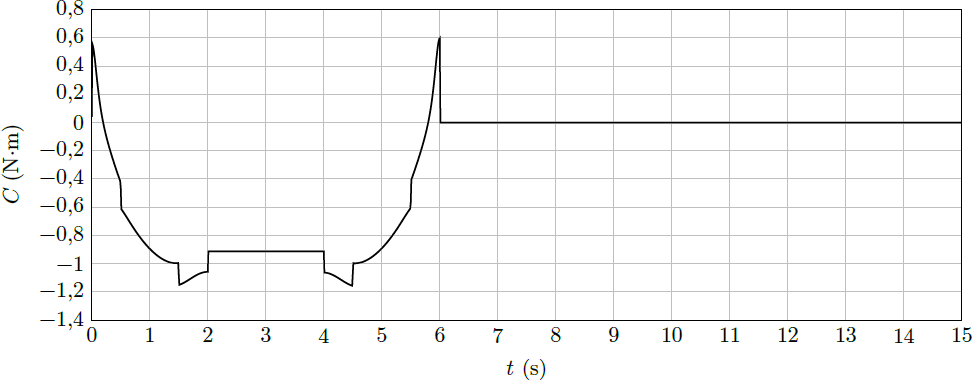
\includegraphics[width=.8\linewidth]{images/fig_12}
%\textit{}
\end{center}


\subparagraph{} \textit{Préciser à quels mouvements correspondent les 4 phases de ce cycle.}

\ifprof
\begin{corrige}
\begin{itemize}
\item Phase 1 : le couple est décroissant, suivant la convention de signe utilisée, on peut faire l'hypothèse que le genou fléchit et que l’accélération est décroissante.
\item Phase 2 : le couple est constant. On peut faire l'hypothèse que le moteur tourne à vitesse constante et que le couple moteur est celui nécessaire à vaincre les frottements. 
\item Phase 3 : le couple est croissant. En conservant la même << convention >> que précédemment, le genou ralentit et arrive en fin de flexion .
\item Phase 4 : si le genou ne bouge plus, on peut faire l'hypothèse que l'exosquelette est en butée. Ainsi, il n'est pas nécessaire d'avoir un couple pour maintenir le système en position.
\end{itemize}
\end{corrige}
\else
\fi

Le couple efficace est également appelé couple thermiquement équivalent, il est défini par :
$C_{\text{eff}}=\sqrt{\dfrac{1}{T}\int\limits_0^Tc(t)^2 \dd t}$. On a aussi 
$C_{\text{eff}}=\sqrt{\dfrac{1}{T}\sum\limits_{i=1}^n C_{\text{i,eff}}^2 T_i }$


\fi

\subparagraph{} \textit{Calculer la valeur efficace du couple moteur du genou pour ce cycle périodique de \SI{15}{s}.}

\ifprof
\begin{corrige}
$C_{\text{eff}}=\sqrt{\dfrac{1}{T}\sum\limits_{i=1}^n C_{\text{i,eff}}^2 T_i }$
$=\sqrt{\dfrac{1}{15}\left(0,838^2 \times 2 +0,912^2 \times 2 + 0,838^2 \times 2 \right) }\simeq \SI{0,546}{Nm}$.
\end{corrige}
\else
\fi


\subsection*{Retour sur l'objectif}

\ifprof
\else

Le couple moteur varie entre \SI{-1,156}{Nm} et \SI{0,596}{Nm}.
Les caractéristiques du moteur choisi sont :
\begin{itemize}
\item vitesse à vide de \SI{3120}{tr.min^{-1}} pour une alimentation nominale en amont de l’onduleur de \SI{36}{V};
\item couple permanent admissible de \SI{0,560}{Nm};
\item pente de la courbe de la vitesse en fonction du couple de \SI{423}{tr.min^{-1}N^{-1}m^{-1}}.
\end{itemize}

De plus une étude cinématique précédente a montré que le moteur permettant d'actionner le moteur doit pouvoir atteindre une vitesse de \SI{2200}{tr.min^{-1}}.

\fi


\subparagraph{} \textit{Conclure quant au choix de ce moteur au regard de la valeur maximale de la vitesse angulaire calculée lors d'une étude précédente et du couple efficace calculé à la question précédente et compléter le schéma bilan.}

\ifprof
\begin{corrige}
\begin{enumerate}
\item Le couple thermiquement équivalent calculé est de \SI{0,546}{Nm} ce qui est inférieur aux couple admissible par le moteur. 
\item La fréquence de rotation à atteindre par le moteur est de \SI{2200}{tr.min^{-1}}. Le moteur proposé tourne à \SI{3120}{tr.min^{-1}} à vide. On peut donc supposer qu'en charge, il atteindre les \SI{2200}{tr.min^{-1}}.
\end{enumerate}
Su ces deux critères le moteur proposé est donc validé. 
\end{corrige}
\else
\fi

\ifprof
\else

\noindent 
\footnotesize
\begin{tabular}{|p{.95\linewidth}|}
\hline
Éléments de corrigé :
\begin{enumerate}
\item .
\item $\vectmc{O_1}{E}{0}\cdot \vect{x_0} = -Lm_4\cos\theta_{10}\dot{h}(t)$.
\item $\vectmd{O_1}{E}{0}\cdot\vect{x_0}=-Lm_4\cos\theta_{10}\ddot{h}(t)$.
\item $ C_r=-m_4 L \cos\theta_{10} \left(g+\ddot{h}(t)\right)\simeq \SI{190,5}{Nm} $. 
\item $C_m\simeq \SI{2,12}{Nm}$.
\item ...
\item ...
\item $C_{\text{eff}} \simeq \SI{0,546}{Nm}$.
\end{enumerate} \\
\hline
\end{tabular}
\normalsize
\fi

\ifprof
\else
\end{multicols}
\fi



\ifprof
\begin{center}
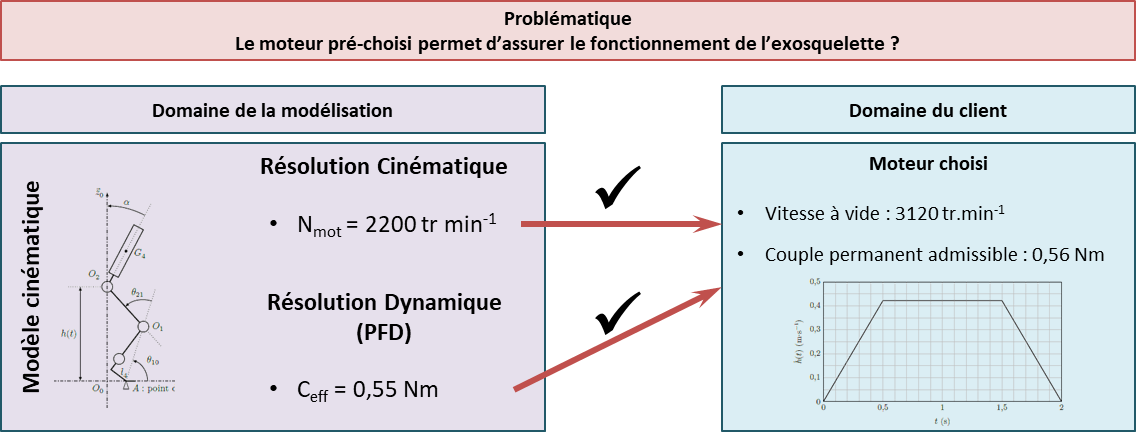
\includegraphics[width=\linewidth]{images/cor_02}
%\textit{}
\end{center}

\else
%\begin{center}
%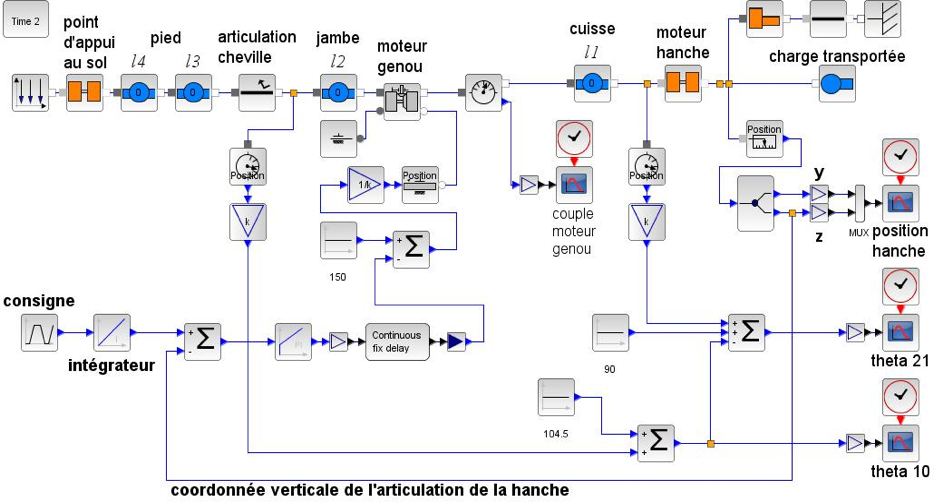
\includegraphics[width=\linewidth]{images/fig_07}
%\textit{}
%\end{center}


\begin{center}
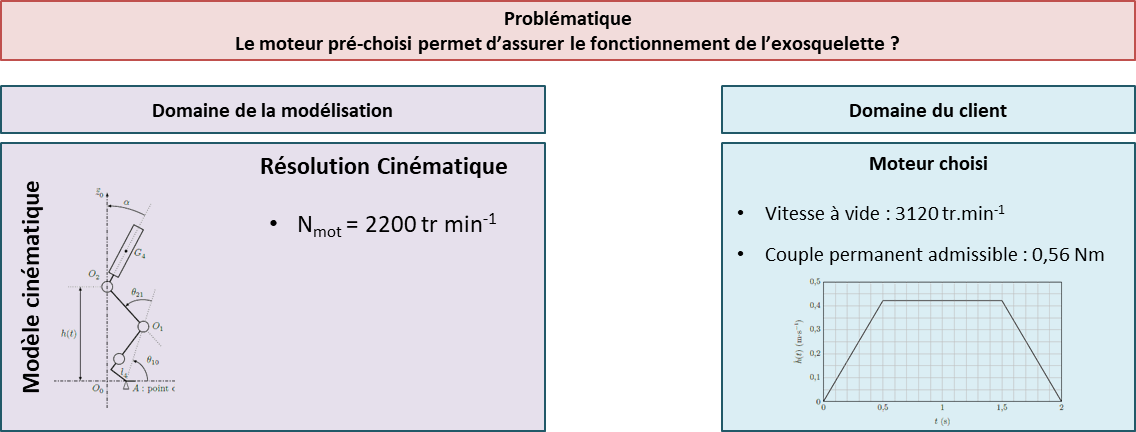
\includegraphics[width=.7\linewidth]{images/fig_15}
%\textit{}
\end{center}
\fi

%\begin{center}
%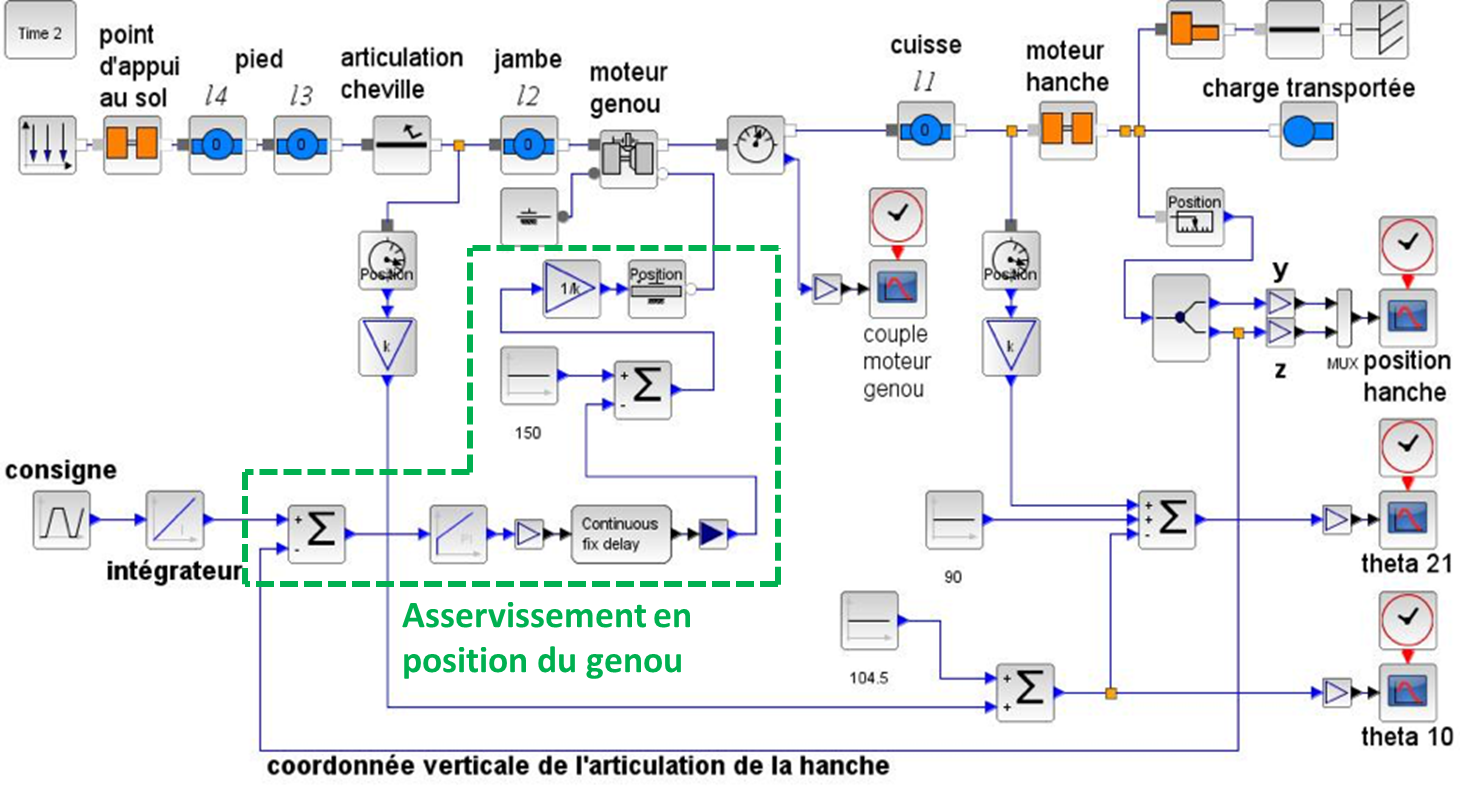
\includegraphics[width=.65\linewidth]{images/cor_01}
%%\textit{}
%\end{center}


